\documentclass[a4paper,11pt]{article}
\usepackage{mathpazo}
\usepackage{tikz}
\usetikzlibrary{shapes}
\oddsidemargin -0.54cm
\textwidth 17.00cm
\textheight 24cm
\topmargin -1.3cm
\parindent 0pt
\parskip 1ex
\pagestyle{empty}
\begin{document}
\medskip\hrule\medskip

5 10 8 6 3 4 2 7 9 1000 are inserted 

In sorted order: 2 3 4 5 6 7 8 9 10 1000 

Average depth = 2.000, size 10

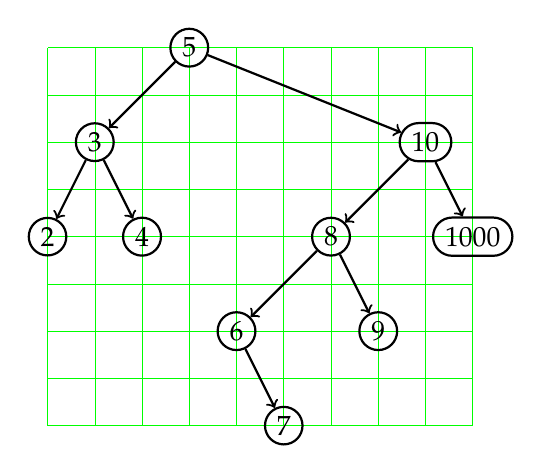
\begin{tikzpicture}[scale=0.600]
\draw [help lines, color=green] (1,-8) grid (10,0);

\draw [thick] (1,-4) node[draw, rounded rectangle] (0) {2};
\draw [thick] (2,-2) node[draw, rounded rectangle] (1) {3};
\draw [thick] (3,-4) node[draw, rounded rectangle] (2) {4};
\draw [thick] (4,0) node[draw, rounded rectangle] (3) {5};
\draw [thick] (5,-6) node[draw, rounded rectangle] (4) {6};
\draw [thick] (6,-8) node[draw, rounded rectangle] (5) {7};
\draw [thick] (7,-4) node[draw, rounded rectangle] (6) {8};
\draw [thick] (8,-6) node[draw, rounded rectangle] (7) {9};
\draw [thick] (9,-2) node[draw, rounded rectangle] (8) {10};
\draw [thick] (10,-4) node[draw, rounded rectangle] (9) {1000};
\draw [->, thick] (1) to (0);
\draw [->, thick] (1) to (2);
\draw [->, thick] (3) to (1);
\draw [->, thick] (3) to (8);
\draw [->, thick] (4) to (5);
\draw [->, thick] (6) to (4);
\draw [->, thick] (6) to (7);
\draw [->, thick] (8) to (6);
\draw [->, thick] (8) to (9);

\end{tikzpicture}

\medskip\hrule\medskip
\end{document}